
\section{Methodology}

\subsection{Data Collection}

Temperature and current data was collected from a motor in a series of data points indexed in time order with temperature and current measurements taken at regular intervals. 

\subsubsection{Temperature sensor}

\begin{figure}[!h]
	\centering
	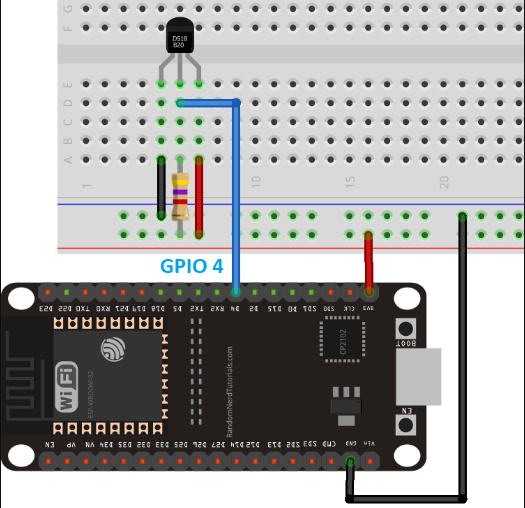
\includegraphics[width=0.7\linewidth, height = 8cm]{Figures/ds18b20}
	\caption{ds18b20 pin out}
	
\end{figure}
To initiate a temperature measurement
and conversion, a read and convert command is issued. Following conversion, the resulting
thermal data is stored in the 2-byte temperature register in the scratchpad memory, to be able to issue this command an external power supply is used to specify read time slots” 

\pagebreak 

\begin{lstlisting}
	void loop() {
		sensors.requestTemperatures(); 
		float temperatureC = sensors.getTempCByIndex(0);
		float temperatureF = sensors.getTempFByIndex(0);
		Serial.print(temperatureC);
		Serial.print(temperatureF);
		Serial.println("F");
		delay(5000);
	}
\end{lstlisting}


\subsubsection{Current sensor}

\begin{figure}[!h]
	\centering
	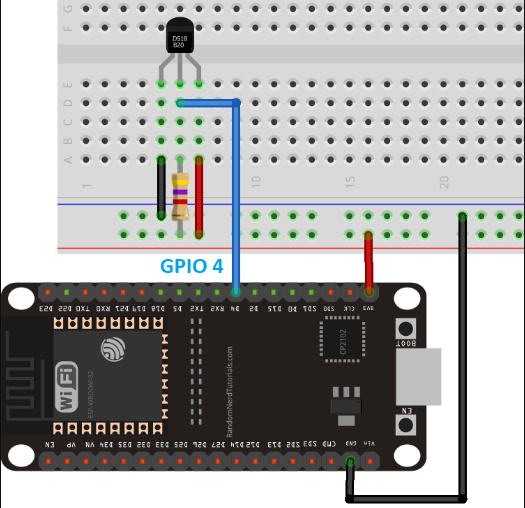
\includegraphics[width=0.7\linewidth, height = 8cm]{Figures/ds18b20}
	\caption{current sensor pin out}
	
\end{figure}
Current flows through the onboard hall sensor circuit in its IC
The hall effect sensor detects the incoming current through its magnetic field generation
Once detected, the hall effect sensor generates a voltage proportional to its magnetic field that’s then used to measure the amount of current 

\begin{lstlisting}
	// The on-board ADC is 10-bits 
	// Different power supply will lead to different reference sources
	// example: 2\^{}10 = 1024 -> 5V / 1024 \~{}= 4.88mV
	//          unitValue= 5.0 / 1024.0*1000 ;
	float unitValue= RefVal / 1024.0*1000 ;
	float voltage = unitValue * sensorValue; 
	
	//When no load,Vref=initialValue
	SERIAL.print(``initialValue: '');
	SERIAL.print(voltage);
	SERIAL.println(``mV''); 
	
	// Calculate the corresponding current
	float current = (voltage - Vref) * sensitivity;
	
	// Print display voltage (mV)
	// This voltage is the pin voltage corresponding to the current
	/*
	voltage = unitValue * sensorValue-Vref;
	SERIAL.print(voltage);
\end{lstlisting} 

\subsubsection{Omnimonitor}

The device is responsible for keeping track of and managing data from different sources as well as managing read and write signals from the sensor to the remotely accessible server  
\begin{figure}[!h]
	\centering
	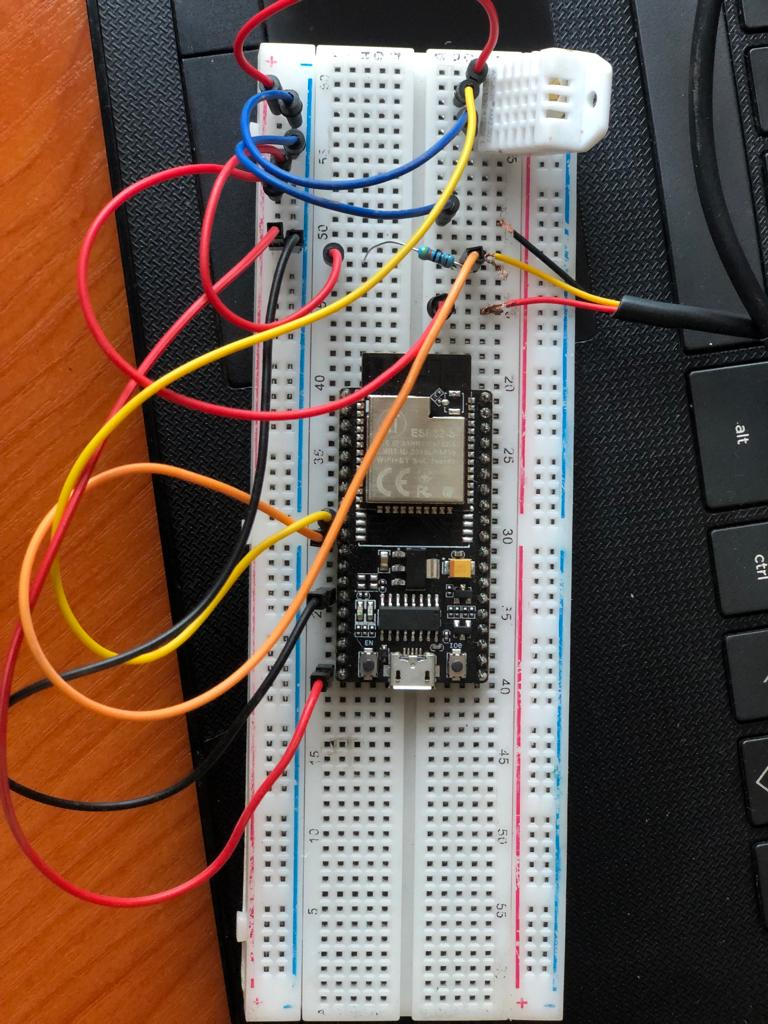
\includegraphics[width=0.7\linewidth, height = 8cm]{Figures/setup}
	\caption{combined sensor setup}
	
\end{figure}
Both ds18b20 and DHT22 provide the output of temperature and humidity in the complex digital output format which can not be directly read with GPIO pins without writing any technique which can read these output signals. These sensors provide data through a single wire two-way communication protocol. A single process communication consists of 40 bits.To get values of temperature and humidity we call a number of created  functions.



\begin{lstlisting}
	\#if defined(ESP32)
	\#include <WiFiMulti.h>
	WiFiMulti wifiMulti;
	\#define DEVICE ``ESP32''
	\#elif defined(ESP8266)
	\#include <ESP8266WiFiMulti.h>
	ESP8266WiFiMulti wifiMulti;
	\#define DEVICE ``ESP8266''
	\#endif
	

	//\#define DHTTYPE DHT11 // DHT 11
	//\#define DHTTYPE DHT21 // DHT 21 (AM2301)
	\#define DHTTYPE DHT22 // DHT 22 (AM2302), AM2321
	
	// ds18b20 sensor
	\#define ONE\_WIRE\_BUS 26
	OneWire oneWire(ONE\_WIRE\_BUS);
	DallasTemperature sensors(\&oneWire);
	
	uint8\_t DHTPin = 25;
	DHT dht(DHTPin, DHTTYPE);
	
	float temperature\_Celsius; // ambient
	float humidity;
	float temperature\_Celcius2; // contact
\end{lstlisting}


\subsubsection{MQTT}

Message Queuing Telemetry Transport (MQTT) is a lightweight messaging protocol designed for usage in situations where clients require a minimal code footprint and are linked to unreliable networks or networks with restricted capacity. It’s mostly utilised for M2M (machine-to-machine) communication and Internet of Things connectivity.  

MQTT uses a PUSH/SUBSCRIBE architecture to run on top of TCP/IP. There are two sorts of systems in MQTT architecture: clients and brokers. The server with which the clients communicate is known as a broker. Client messages are received by the broker, who then forwards them to other clients. Clients connect to the broker rather than communicating directly with one another.

MQTT also reduces transmissions by using a well-defined, compact message structure. In comparison to HTTP, each message has a fixed header of only 2 bytes.


\subsubsection{OTA}

Instead of needing the user to connect the ESP32 to a computer via USB to execute the update, OTA programming allows update of new data to the ESP32 via Wi-Fi.

When there is no physical access to the ESP module, the OTA capability comes in handy. It helps to cut down on the time spent on each ESP module during maintenance.

One of the most useful features of OTA is that it allows a single central location to deliver an update to many equipment on the same network ideally all monitored equipment in a ship engine room.

\subsubsection{Declaration, definition and initialization}

Define, declare variables and initialize classes. 

\begin{lstlisting}
	#define CURRENT_VERSION "1.0.0" // The current version of the firmware running
	#define DOWNLOAD_URL SERVER_URL // The server url where we will get the latest firmware version
	#define DHTPIN 2 // Digital pin connected to the DHT sensor
	#define DHTTYPE DHT11 // DHT 11
	#define LED 4 // Digital pin connected to the inbuilt LED
	WiFiClient espClient; //Initializing the WiFiClient
	void setup_wifi();
	void reconnect();
	PubSubClient client(espClient); // Initializing the PubSubClient
	WebServer server(80); // Initializing the WebServer
	// functions to take care of OTA firmware update
	void handleRoot();
	String getDownloadUrl();
	bool downloadUpdate(String);
	DHT_Unified dht(DHTPIN, DHTTYPE);
	int ledState = LOW; // Set the ledstate to be off at the first instance
	const long interval = 1000; // This is the interval we will be using to check for a new version
	unsigned long previousMillis = 0; // previous timings in milliseconds
	unsigned long currentMillis; // current timings in milliseconds
	bool success; // download success
	
\end{lstlisting}

\subsubsection{Setup function}

This is  executed only once in the beginning of the program.



\begin{lstlisting}
	void setup() \{
	Serial.begin(115200); // begin Serial at 115200 baud rate
	setup\_wifi(); // function to setup up wifi
	espClient.setServer(mqtt\_server, 1883); //Setup the MQTT server
	
	// Initialize device.
	dht.begin();
	// Print temperature sensor details.
	sensor\_t sensor;
	dht.temperature().getSensor( \& sensor);
	Serial.println(F(`));
	Serial.println(F(``Temperature Sensor Present''));
	
	// Print humidity sensor details.dht.humidity().getSensor(\&sensor);
	Serial.println(F(`` ));
	Serial.println(F(``Humidity Sensor Present''));
	Serial.setDebugOutput(true); // Set debug to true in order to print more serial output
	pinMode(LED, OUTPUT); // Initialize the inbuilt led as an output device
	delay(3000); // Set a delay of 3 seconds (optional)
	String version = String(``<p>Current Version - v'') + String(CURRENT\_VERSION) + String(``</p>'');
	Serial.println(version);
	// Setup Wifi Manager
	WiFiManager wm;
	WiFiManagerParameter versionText(version.c\_str());
	wm.addParameter( \& versionText);
	if (!wm.autoConnect()) \{
	Serial.println(``failed to connect and hit timeout'');
	ESP.restart();
	delay(1000);
	\}
	// Check if we need to download a new version
	String downloadUrl = getDownloadUrl();
	if (downloadUrl.length() > 0) \{
	success = downloadUpdate(downloadUrl);
	if (!success) \{
	Serial.println(``Error updating device'');
	\}
	\}
	server.on(``/'', handleRoot);
	server.begin();
	Serial.println(``HTTP server started'');
	Serial.print(``IP address: '');
	Serial.println(WiFi.localIP());
	\}
\end{lstlisting}
\subsubsection{Loop function}
This section is repeated after a specified interval to read and write parameters specified
\begin{lstlisting}
	// Get temperature event and print its value.
	sensors_event_t event;
	dht.temperature().getEvent( & event);
	if (isnan(event.temperature)) {
		Serial.println(F("Error reading temperature!"));
	} else {
		Serial.print(F("Temperature: "));
		Serial.print(event.temperature);
		Serial.println(F("°C"));
	}
	// Get humidity event and print its value.
	dht.humidity().getEvent( & event);
	if (isnan(event.relative_humidity)) {
		Serial.println(F("Error reading humidity!"));
	} else {
		Serial.print(F("Humidity: "));
		Serial.print(event.relative_humidity);
		Serial.println(F("%"));
	}
	currentMillis = millis();
	if (currentMillis - previousMillis >= interval) {
		previousMillis = currentMillis;
		ledState = ledState == LOW ? HIGH : LOW;
		digitalWrite(4, ledState);
	}
	// Just chill
	server.handleClient();
	delay(1000);
	char msg[200];
	if (!espClient.connected()) {
		reconnect();
	}
	StaticJsonBuffer < 300 > JSONbuffer;
	JsonObject & JSONencoder = JSONbuffer.createObject();
	JSONencoder["time"] = millis();
	JSONencoder["temperature"] = event.temperature;
	JSONencoder["humidity"] = event.relative_humidity;
	char JSONmessageBuffer[100];
	JSONencoder.printTo(JSONmessageBuffer, sizeof(JSONmessageBuffer));
	Serial.println(JSONmessageBuffer);
	if (espClient.publish("dht/user_id892", JSONmessageBuffer) == true) {
		Serial.println("Success sending message");
	} else {
		Serial.println("Error sending message");
	}
	espClient.loop();
}

\end{lstlisting}


\subsubsection{Handle server requests}
Ensures data is read only when it can be written to the server. 
\begin{lstlisting}
	void handleRoot() {
		server.send(200, "text/plain", "v" + String(CURRENT_VERSION));
	}
	
\end{lstlisting}
\subsubsection{Download links}

\begin{lstlisting}
	String getDownloadUrl() {
		HTTPClient http;
		String downloadUrl;
		Serial.print("[HTTP] begin…\n");
		String url = DOWNLOAD_URL;
		http.begin(url);
		Serial.print("[HTTP] GET…\n");
		// start connection and send HTTP header
		int httpCode = http.GET();
		// httpCode will be negative on error
		if (httpCode > 0) {
			// HTTP header has been send and Server response header has been handled
			Serial.printf("[HTTP] GET… code: %d\n", httpCode);
			// file found at server
			if (httpCode == HTTP_CODE_OK) {
				String payload = http.getString();
				Serial.println(payload);
				downloadUrl = payload;
			} else {
				Serial.println("Device is up to date!");
			}
		} else {
			Serial.printf("[HTTP] GET… failed, error: %s\n", http.errorToString(httpCode).c_str());
		}
		http.end();
		Serial.println(downloadUrl);
		return downloa
	
\end{lstlisting}
\subsubsection{Download binary firmware }
 This is used to 
\begin{lstlisting}
	/*
	Download binary image and use Update library to update the device.
	*/
	/*
	Download binary image and use Update library to update the device.
	*/
	bool downloadUpdate(String url) \{
	HTTPClient http;
	Serial.print(``[HTTP] Download begin…\textbackslash{}n'');
	http.begin(url);
	Serial.print(``[HTTP] GET…\textbackslash{}n'');
	// start connection and send HTTP header
	int httpCode = http.GET();
	if (httpCode > 0) \{
	// HTTP header has been send and Server response header has been handled
	Serial.printf(``[HTTP] GET… code: \%d\textbackslash{}n'', httpCode);
	// file found at server
	if (httpCode == HTTP\_CODE\_OK) \{
	int contentLength = http.getSize();
	Serial.println(``contentLength : '' + String(contentLength));
	if (contentLength > 0) \{
	bool canBegin = Update.begin(contentLength);
	if (canBegin) \{
	WiFiClient stream = http.getStream();
	Serial.println(``Begin OTA. This may take 2–5 mins to complete. Things might be quite for a while.. Patience!'');
	size\_t written = Update.writeStream(stream);
	if (written == contentLength) \{
	Serial.println(``Written : '' + String(written) + `` successfully'');
	\} else \{
	Serial.println(``Written only : '' + String(written) + ``/'' + String(contentLength) + ``. Retry?'');
	\}
	if (Update.end()) \{
	Serial.println(``OTA done!'');
	if (Update.isFinished()) \{
	Serial.println(``Update successfully completed. Rebooting.'');
	ESP.restart();
	return true;
	\} else \{
	Serial.println(``Update not finished? Something went wrong!'');
	return false;
	\}
	\} else \{
	Serial.println(``Error Occurred. Error \#: '' + String(Update.getError()));
	return false;
	\}
	\} else \{
	Serial.println(``Not enough space to begin OTA'');
	client.flush();
	return false;
	\}
	\} else \{
	Serial.println(``There was no content in the response'');
	client.flush();
	return false;
	\}
	\} else \{
	return false;
	\}
	\} else \{
	return false;
	\}
	\}
	
\end{lstlisting}
\subsubsection{Setup wifi function}

\begin{lstlisting}
	void setup_wifi() {
		// Connecting to a WiFi network
		WiFi.begin(ssid, password);
		while (WiFi.status() != WL_CONNECTED) {
			delay(500);
			Serial.print(".");
		}
		Serial.println("WiFi connected");
		Serial.println("IP address: ");
		Serial.println(WiFi.localIP());
	}
	
\end{lstlisting}
\subsubsection{Reconnect function}

\begin{lstlisting}
	void reconnect() {
		// Loop until we're reconnected
		Serial.println("In reconnect…");
		while (!espClient.connected()) {
			Serial.print("Attempting MQTT connection…");
			// Attempt to connect
			if (espClient.connect("SES_DHT", MQTT_USER, MQTT_PASS)) {
				Serial.println("connected");
			} else {
				Serial.print("failed, rc=");
				Serial.print(espClient.state());
				Serial.println(" try again in 5 seconds");
				delay(5000);
			}
		}
	}
	
\end{lstlisting}

\subsection{Data Analytics Process Steps}
 
The motor sensors output digital and analogue electrical signals. This is parsed to literal temperature and current values i.e degrees and amperes respectively. 
This is automated by use of a C bash script that then data is written into a CSV file that is now the accessible database for the algorithm fetch requests. 

The data is prepared for analysis by wrangling to remove unwanted and redundant values. The stage is now set to visualize the data to be able to observe meaningful patterns that can provide useful insights to the motors condition. Ultimately this will also provide the logical descriptive equations on which predictive algorithms will learn from.

To prove meaningful results tests were developed to check if the output is in line with the expected results


\begin{figure}[hb]
	\centering
	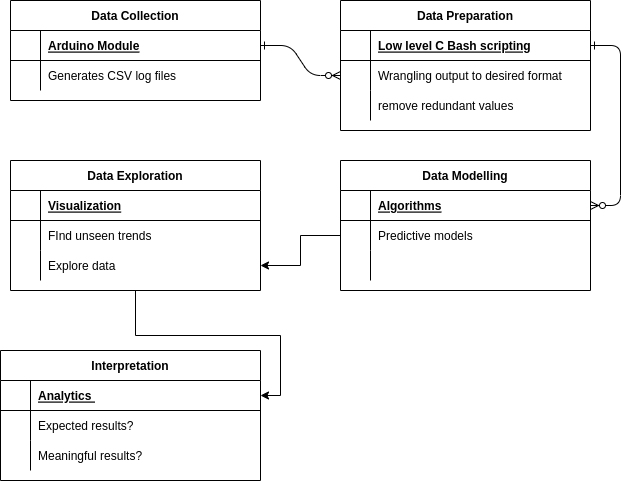
\includegraphics[width=0.7\linewidth]{Figures/data_analytics_process-steps}
	\caption{Data Analytics}
	\label{fig:dataanalyticsprocess-steps}
\end{figure}


\subsection{ Data Analysis}
The data collected from the sensors will be analyzed using custom software created using vim. Graphs will be generated to compare the performance of each component.

\begin{lstlisting}
	DallasTemperature::request_t DallasTemperature::requestTemperatures() {
		DallasTemperature::request_t req = {};
		req.result = true;
		
		_wire->reset();
		_wire->skip();
		_wire->write(STARTCONVO, parasite);
		
		// ASYNC mode?
		req.timestamp = millis();
		if (!waitForConversion)
		return req;
		blockTillConversionComplete(bitResolution, req.timestamp);
		return req;
	}
\end{lstlisting}


	\subsubsection{Descriptive analysis}
	Using exploratory data analysis prior and current running status is determined 
	
	\subsubsection{Predictive analysis}
	Achieved by building predictive models. The required replacement parts as well as time required for maintenance can be determined.
	
	\subsubsection{Prescriptive analysis}
	This will provide insights on how to create desired outcomes i.e reduce load by 5\% for increased service life 
	
\subsection{System Modelling}

The predictive maintenance algorithm for motors system will be obtained from governing
equations from which a transfer function will be generated from the linearized model. The
transfer function will be used to generate a state space model for the system.
The observed sources of faults and their relative frequency. Such sources can be the core
components of the machine or its various sensors (such accelerometers and flow meters).
The process measurements through sensors. The number, type and location of sensors,
and their reliability and redundancies all will create both algorithm and comparative
model.
The sources of faults will translate to observed symptoms. Such cause-effect analysis will
require extensive processing of data from the available sensors.
Physical knowledge about the system dynamics will result in mathematical modeling of
the system and its faults and from the insights of data. Understanding system dynamics
will involve detailed knowledge of relationships among various signals from the machinery
(such as input-output relationships among the actuators and sensors), the machine operating
range, and the nature of the measurements (for example, periodic, constant or stochastic).
The ultimate maintenance goal, such as fault recovery or development of a maintenance
schedule




\subsection{ Sensors}
Sensors will be used to collect data from the system as it runs. These include:
\begin{enumerate}
	\item Humidity sensor
	\item Temperature sensor
	\item Flow rate sensor
	\item Pressure sensors
	\item Voltage sensor
	\item Current sensor
	
	These sensors will be used by the controller to observe system performance and optimize for each parameter.
\end{enumerate}

\subsection{ Process chart}
From the generated models on, simulations will be performed using the different
controllers and the responses and other metrics will be plotted out for further analysis using NumPy and Pandas python libraries .
Values such as rise time, settling time and stochastic response will be observed to determine the system performance.
\begin{figure}
	\centering
	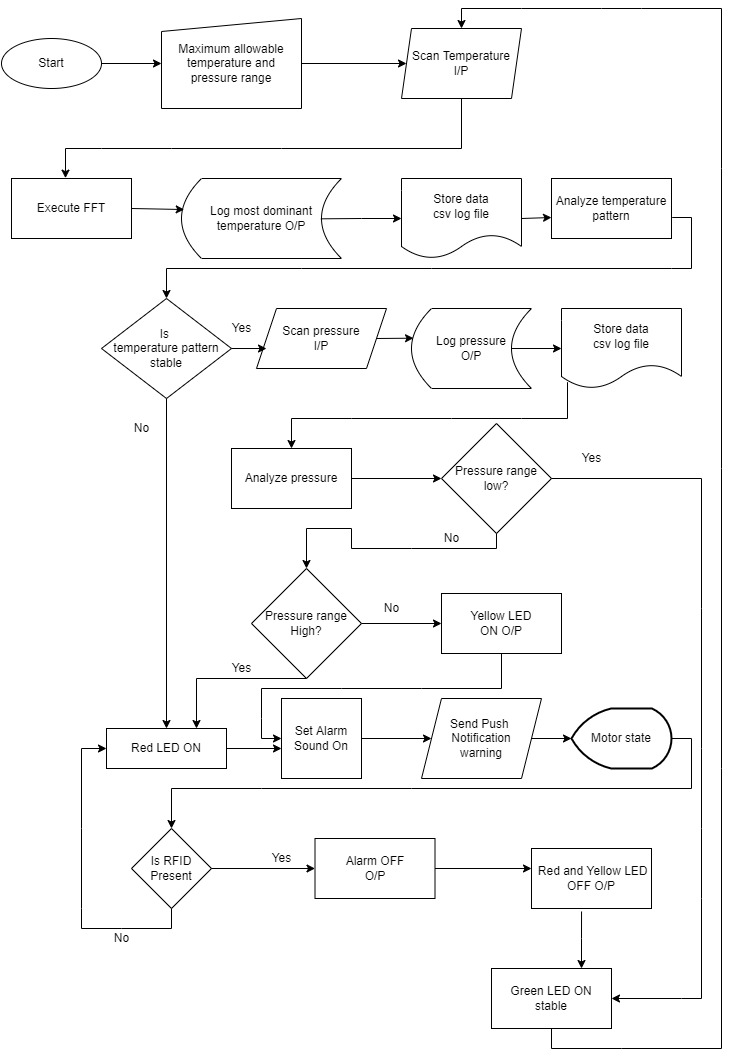
\includegraphics[width=0.7\linewidth]{Figures/model1}
	\caption{Module Process}
	\label{fig:model1}
\end{figure}


%\subsubsection{External Force Sensor}

%\subsubsection{Stewart Platform as a force sensor}
